\chapter{Courses 2 LMS}
\label{sec:courses}

Now, that we have understaning of how CodeIgniter works, we can continue with description of Courses 2 system, as it was developed by Jakub Culik \cite{culik}. Goal of this chapter is to describe this system as it was implemented before this work, explain motivation for creating a new Learning Management System (LMS) and bring some technical details of Courses 2 LMS, which are important for future understandings of this work.

\section{Motivation}

Courses 2 system was developed during spring and winter of 2015 with development team led by Jakub Culik. This team was able to create a simple, customizable and modular learning management system which is already used at our faculty. Until the end of summer semester of 2016, 32 courses with total of 200 students were using this system.


Need for this system started in 2010, when a new aproach of the learning was introduced in the web design course at our faculty \cite{culik}. Each student had to publish a multiple blog posts which where then evaluated by his classmates and  the teachers. Ratings were later projected into his final grade from this course. This approach led students to study more about topics they were interested in and were related to this subject. With this approach, students were also forced to discuss these problems and got a greater insight into related topics.

The portal we used, \texttt{blog.matfyz.sk} was also developed at our faculty in 2008 by Martin Rejda \cite{rejda}, so there were many options improve this system and to modify it to our needs. For example, blog portal was modified to allow students to implement and submit their own blog layout in XSLT. Hovewer, there were still some missing features like system for reviewing of these blog articles and discussions so the need for another system arose \cite{culik}. As a solution, new system, Courses was created \cite{culikbc}.


This system was developed as a part of bachelor's thesis in 2013 \cite{culikbc} and was running 4 courses for one year \cite{culik}. After this time, it seemed clear that this system has to be completely redesigned and implemented from scratch. A new system had to be modular, scalable and well designed. And this is how Courses 2 was born.

\section{Semantics}

Courses 2 system architecture can be divided into two parts: system part and modules. This division is required for maintaining this system modular and scalable. Now, let's look at each part.

\subsection{System}

System part is mostly responsible for "background stuff". Models and controllers extend standard CodeIgniter classes and there is only a few standalone libraries. All files of this part are located in \texttt{application/} folder and comply with standard CodeIgniter MVC flow.


Main goal of this part is to share basic data to every component. For example, after a user logs in, user information have to be available for each module. Since Course and Layout information are shared too, it is placed here as well. This part is also responsible to decide which modules has to be run on specific request and printing their outputs on the correct place in application layout.

\subsection{Modules}

After the system part is initialized, correct modules has to be run. Currently, there are 5 modules installed: \texttt{Core}, \texttt{Assignments}, \texttt{Quiz}, \texttt{Notes}, \texttt{Results}. Each module has different purpose and we will later explain \texttt{Assignments} throughoutly as it is main focus of this work. Other modules work similar and are not referenced by us, so we do not consider their description important for this work.

\subsection{Layout}

Layout is managed by system part of this application. CodeIgniter default layout system is not sufficient for required modularity, so it had to be replaced by a new one. Main problem was that each part of layout can be rendered by different module, which is decided at run-time. So page structure was divided into 4 different parts, each with its own rendering.


Courses 2 is build to offer one, root layout for all of the pages. This layout is located in \texttt{application/views} directory of the project.

\begin{figure}[h]
    \centering
    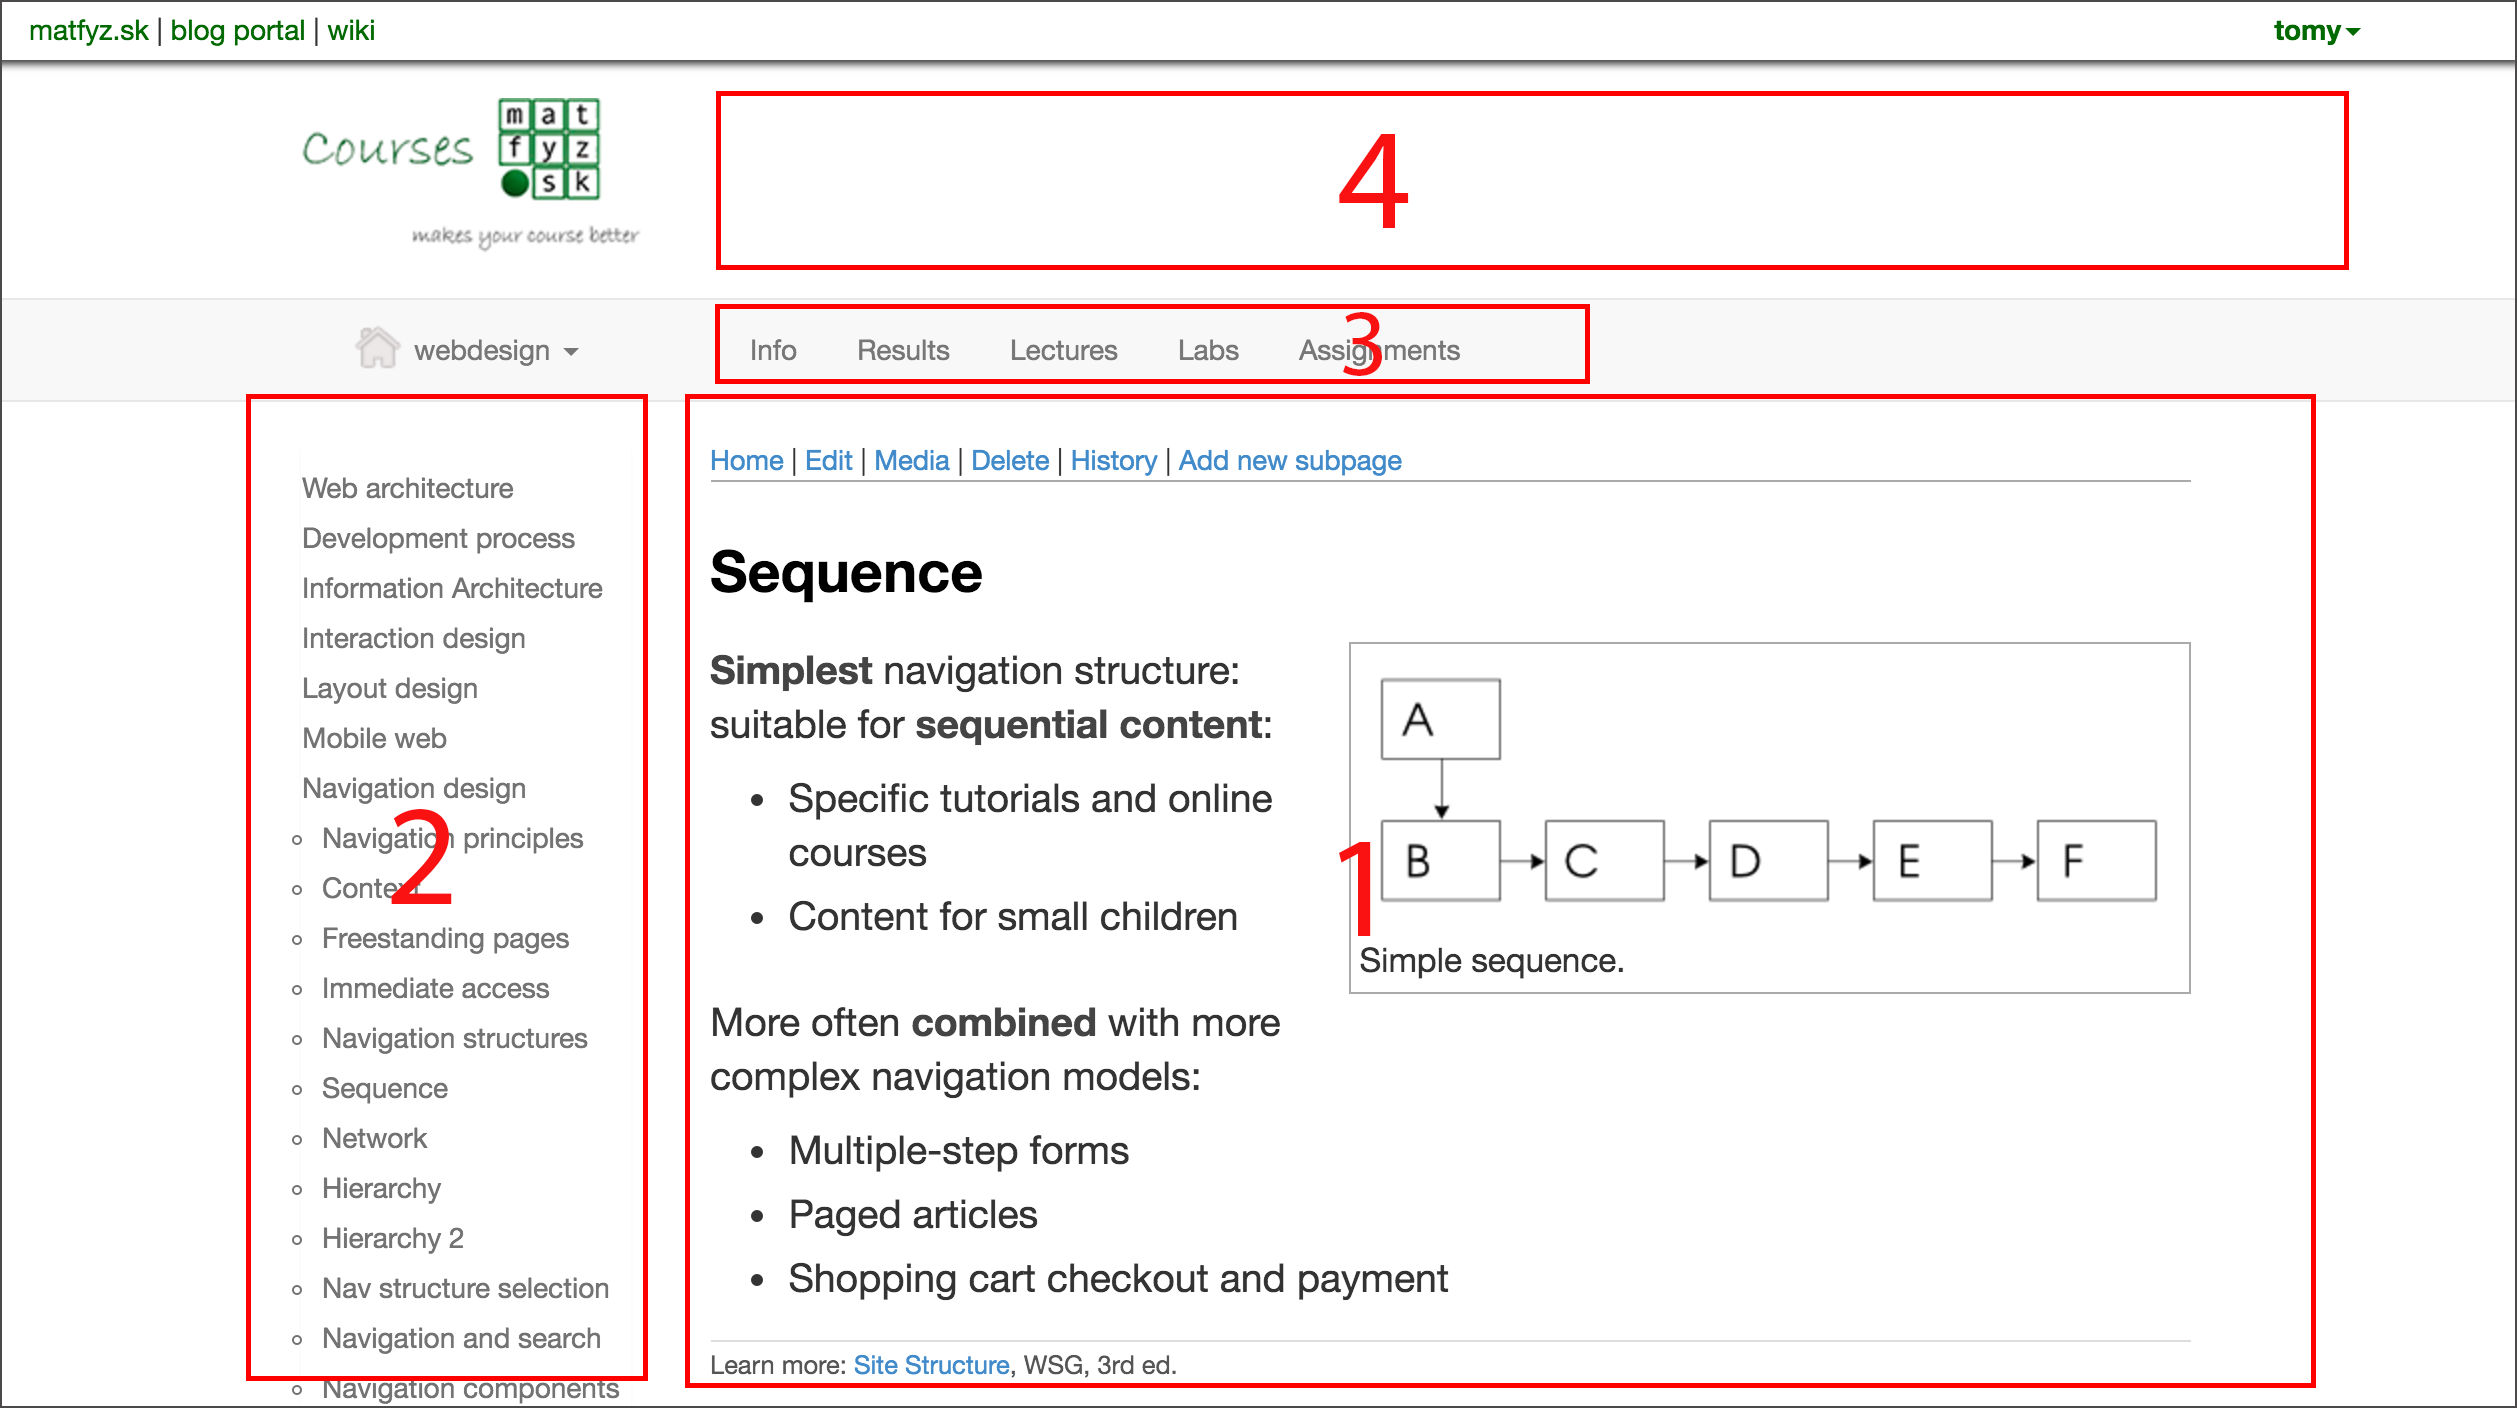
\includegraphics[width=0.95\textwidth]{images/courses-labelled.png}
    \caption{Courses 2 screenshot}
    \label{courses2screen}
\end{figure}


As shown on figure \ref{courses2screen}, root layout was split into 4 different parts, each with specific purpose and is rendered independently. Each numbered part is rendered by selected module, the rest is rendered by system. This screenshot was created using \texttt{Notes} module while it showed the content of a lecture. Part number 4 is reserved for user notifications.

\section{HMVC extension}
Using MVC design pattern is excellent for building small applications. Hovewer, huge application building on pure MVC pattern brings also some disadvantages \cite{culik}. For example, large sets of views, models and controllers could be a point of failure for many programmers. These sets of classes easily get messed up and chaotic. Hierarchical Model-View-Controller tries to bring an order into this mess.\cite{hmvc}.

HMVC is a direct extension of the MVC pattern that aims to solve mainly scalability issues mensioned earlier. HMVC was first described in a blog post on the JavaWorld web site in July 2000 \cite{hmvc}. In summary, HMVC is a collection of MVC triads operating as one application. By the term triad, we mean single instance of MVC serving for one specific function. Each of this triads then is treated as individual and can be rendered on its own. This resolves into greater scalability, code reusability and most importantly, resolves the problem with hudge views in large projects.

To successfuly implement HMVC, it is crucial for application to be broken into systems \cite{hmvc}. Each system has its own views, models and controllers and is responsible for its own part and nothing else. In Courses 2 system, these systems are called modules, which we will discuss later. One of the advantages of using HMVC design pattern is, that we can focus on one module without changes in implementation of others.

To add support for HMVC in CodeIgniter, we needed to customize this framework. In our predecessive work Modular Extensions \cite{modularextensions} was selected. One of the reasons for usage of this extensions was that in CodeIgniter we can no instantiate more than 1 controller per request. Therefore, to achieve HMVC, we have to simulate these controllers \cite{modularextensions}. 

Modular extensions allow us to call subcontrollers in controllers, but these subcontrollers must extend \texttt{MX\_Controller} class instead of \texttt{MI\_Controller} class. Another difference is that all autoload files has to  be specified in subcontroller and are no longer autoloaded by default. This differences are shown on listing \ref{modularcontroller}.

\begin{lstlisting}[label={modularcontroller}, caption={Module controller}]
<?php     
class Module_controller extends MX_Controller 
{
    $autoload = array(
        'helper'    => array('escape', 'form'),
        'libraries' => array('email'),
    );
}
\end{lstlisting}


With this extension, all modules has are placed in \texttt{application/modules} directory and can be called by base CodeIgniter controller.

\section{Assignments Module}

Now, we will describe the Assignments module, whose development aims to be core of this work. We will provide description as it existed before publishing this work and before any development to the module was made. We consider this section to be important for differentiating our work from what has been done.

Originally, Assignments module was developed for submitting blog posts with the ability for users to review them. However  this idea quickly shifted to more complex module which provides multiple types of interfaces for managing student homework, file or URL submissions and student reviews. This module can be divided into two parts.

\subsection{Student's part}

Student's part did not offer a lot of functionality, it had been designed to be as simple as possible. It quickly became a point of complaints for some students and later in this work we redesigned the user interface. As seen on figure \ref{assstudent}, this interface was way too minimalistic which could lead to missing some important deadlines.

\begin{figure}[h]
    \centering
    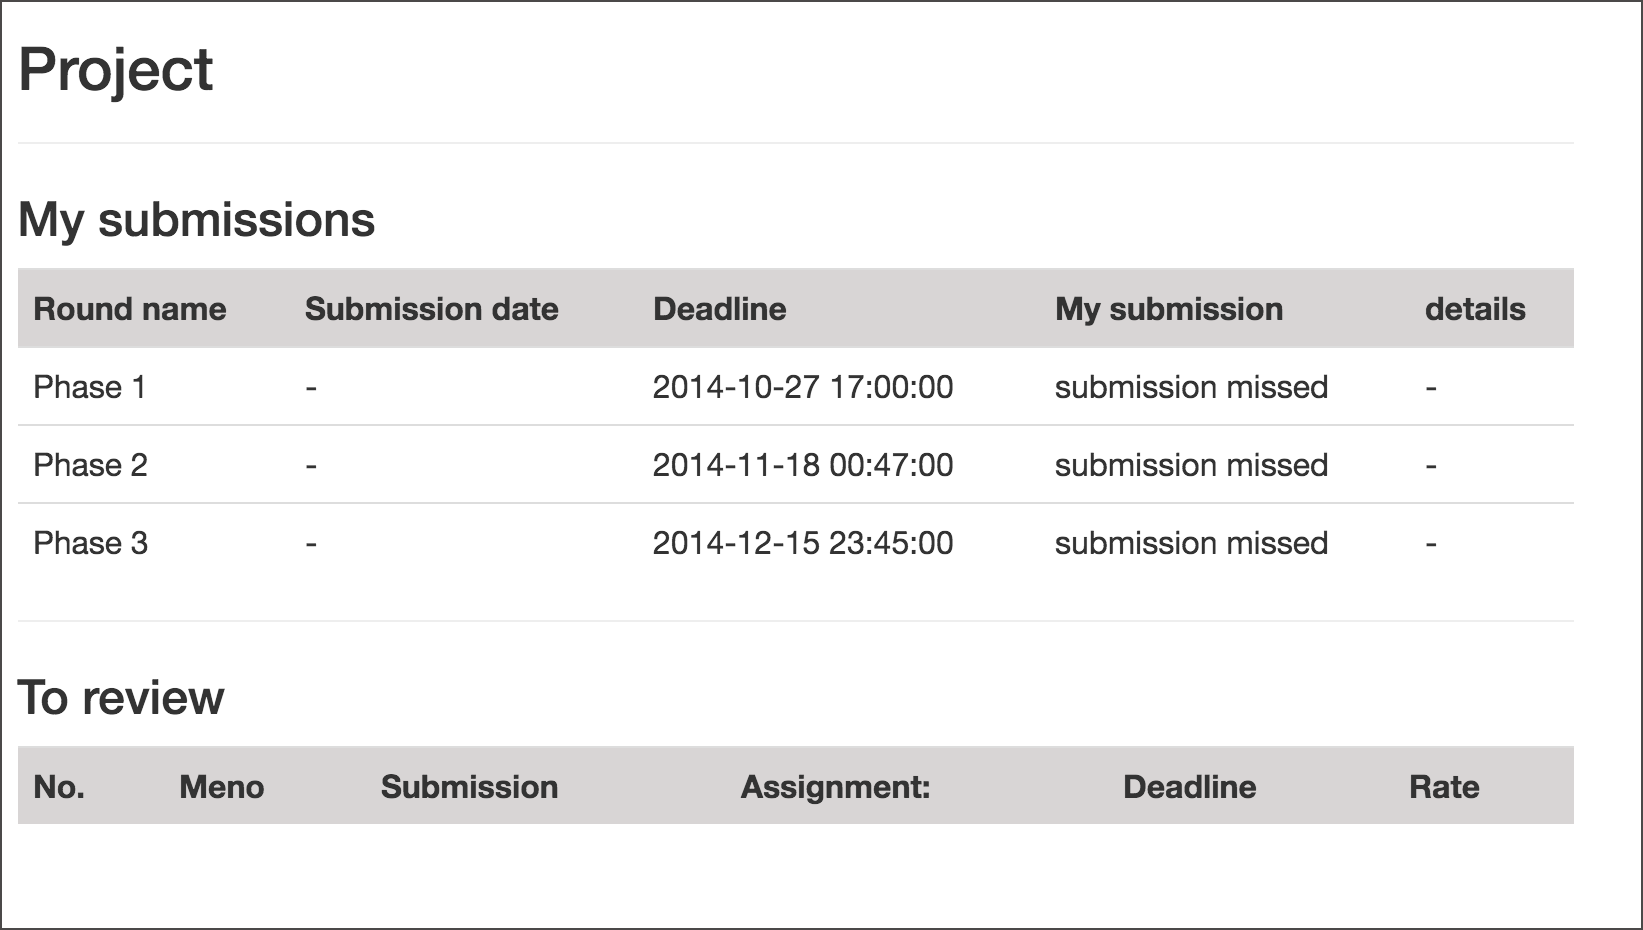
\includegraphics[width=0.95\textwidth]{images/assstudent.png}
    \caption{Student's part of assignment module}
    \label{assstudent}
\end{figure}


This part offered three important functionalities. First was that student can submit his homework assignment with added support for multiple assignment rounds. This means that each assignments can consist of multiple rounds of submissions. For example in first round of an assignment, student must complete 50\% of selected tasks and in second round all of the tasks have to be completed. Second important functionality was peer reviewing of each round. After student submits a submission, other students can see it and write their feedback to this student. These feedback are often also evaluated and projected into final grade of the course. Third functionality was viewing evaluations from teacher and classmates.

\subsection{Teacher's part}

This interface was more complex than previous. It consisted of multiple screens, some of them are presented on figure \ref{teachereval} and \ref{teacherrounds}. This interface also provided two important functionalities: assignment and review operations (create assignment, assign reviews on submitted assignments, delete assignment, edit assignment) and evaluation (assignments and reviews).



\begin{figure}[h]
    \centering
    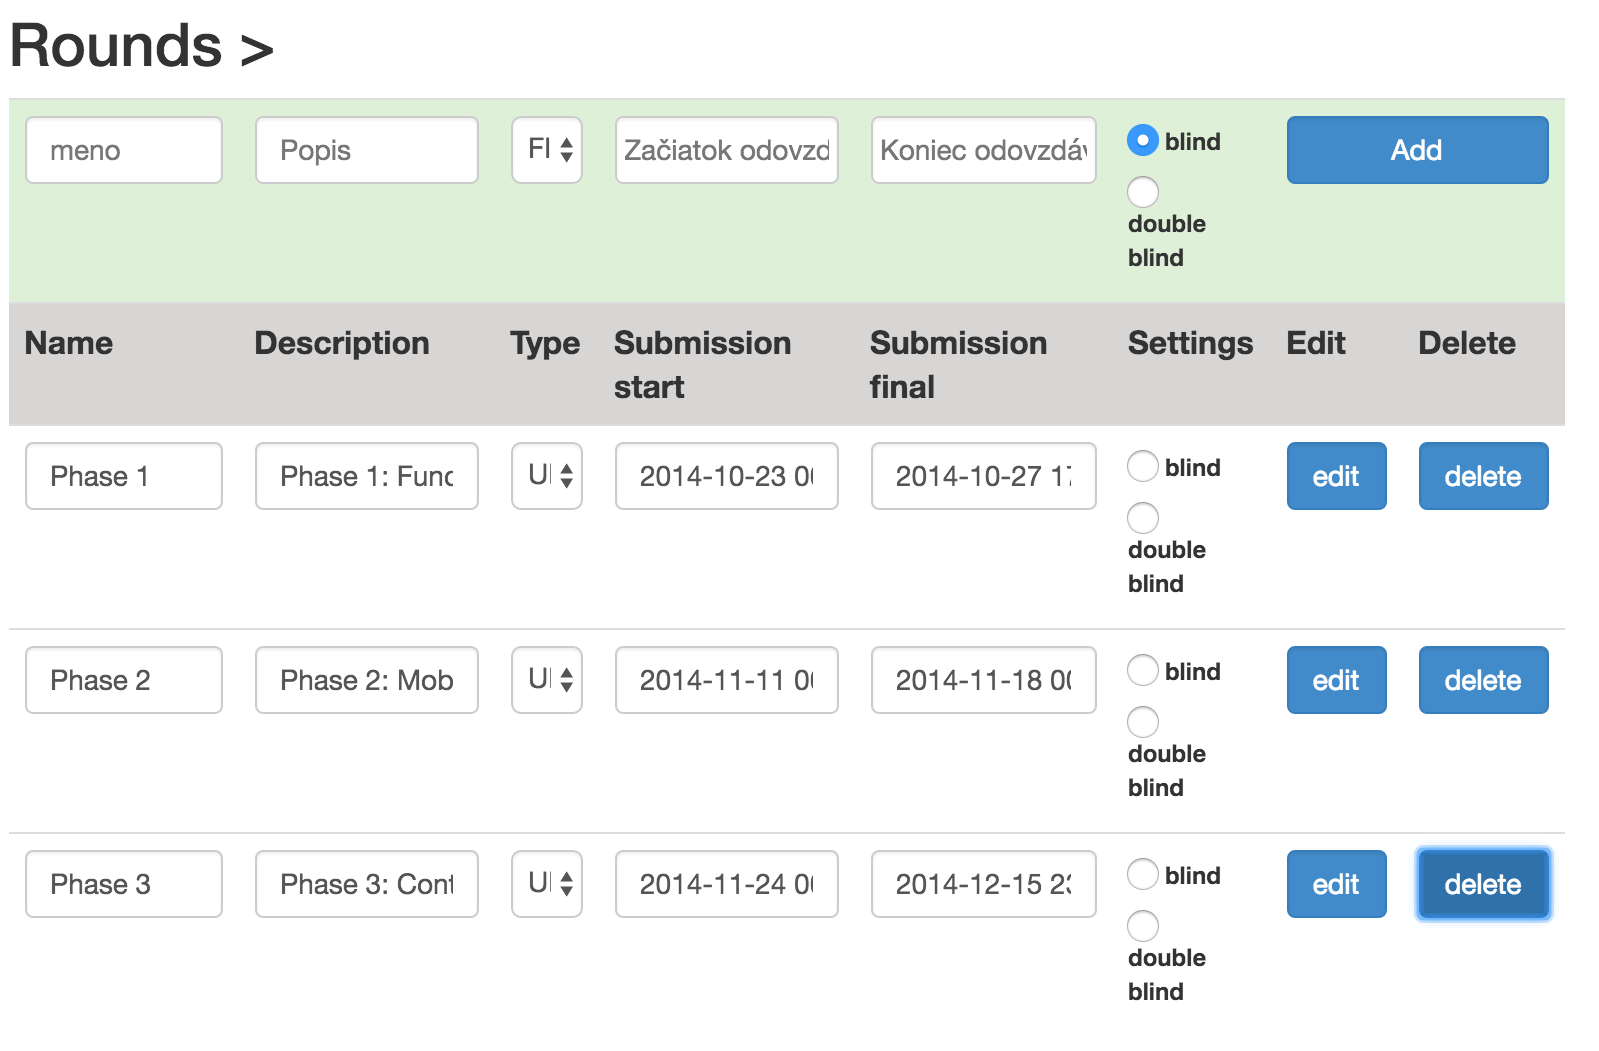
\includegraphics[width=0.95\textwidth]{images/teacherrounds.png}
    \caption{Teacher's administration of assignment rounds}
    \label{teacherrounds}
\end{figure}


On figure \ref{teacherrounds} is shown an Assignment round management. It was possible to set the name of an assignment, set its description (which may provide some instructions for students), type (URL of FILE), submission deadlines and reviewing settings. It was also possible to set student review deadlines, questions and ratings.

\begin{figure}[h]
    \centering
    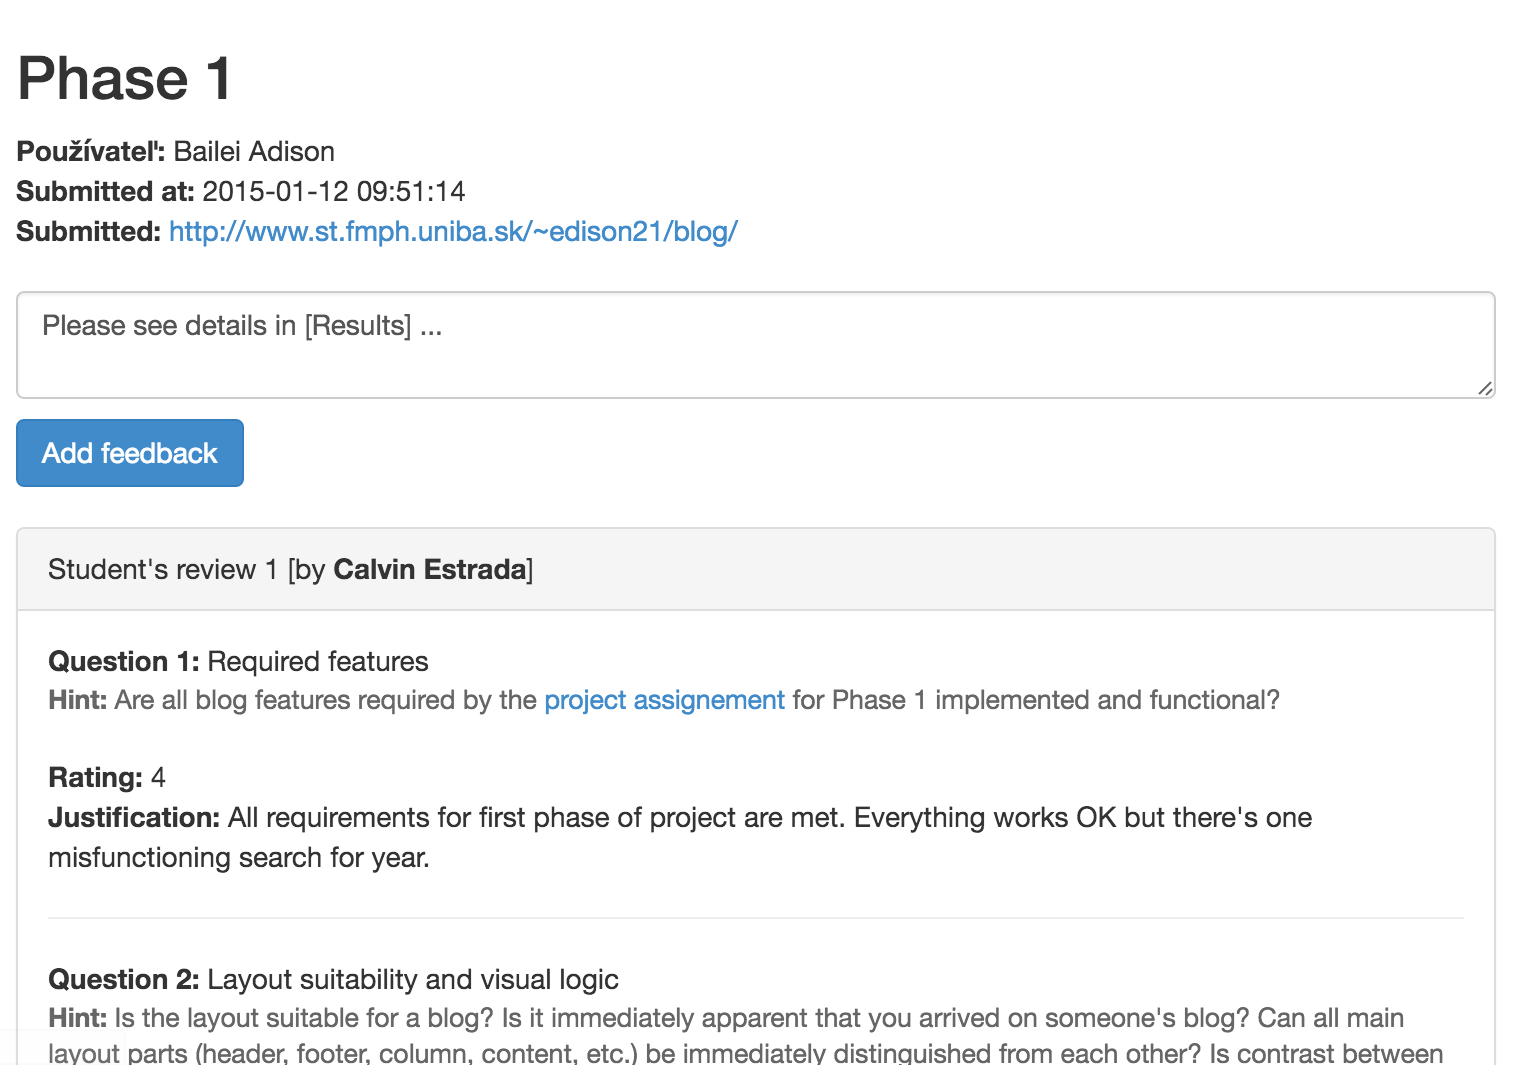
\includegraphics[width=0.95\textwidth]{images/teachereval.png}
    \caption{Teacher's evaluation of submitted assignments}
    \label{teachereval}
\end{figure}


On figure \ref{teachereval} we can see the teacher's evaluation screen. Each round of a submitted assignment is presented on its own screen. The teacher is allowed to submit his own comment to this assignment and evaluate this assignment. There are also shown other student's reviews for this particular round of assignments. 

\section{Implementation}

Whole module is located in \texttt{application/modules/assignment} folder with file structure as described by CodeIgniter Modular Extensions. Now we describe the code flow of this module.


At first, as soon as system part of Courses 2 finds out that assignment module has to be run, routing of this script takes part. All routes are located in \texttt{application/modules/assignment/routes.php}. This script also loads correct course from database and acts as a "bootloader". After correct controller is selected from routing, it is instantiated and run.

\begin{lstlisting}[label={assrouting}, caption={Routing in assignments module for administrator}]
if (is_admin())
{
    switch (url_segment(3))
    {
        case false:
            $route['assignments'] = 'user/assignments';
            break;
        case 'admin':
            $route['assignments'] = 'admin/assignments';
            break;
        case 'reviews':
            $route['assignments'] = 'admin/manage_reviews';
            break;
        default:
            $route['assignments'] = 'admin/manage_assignments';
    }

    return;
}
\end{lstlisting}


After end of Jakub Culik's \cite{culik} work, there were 6 controllers in this module. 3 of them were used for teacher's administration and 3 were used for student's part. All controllers extend \texttt{Module\_Controller} class and implement \texttt{Module\_Interface}, which is special superclasses for all modules controllers.

Models are located in \texttt{application/modules/assignment/models/} and views in \texttt{application/modules/assignment/views}. As seen on listing \ref{assviews} there are multiple languages, such as HTML, PHP or CSS used.

\begin{lstlisting}[label={assviews}, caption={Example of view in assignments module}]
<h2><?= lang('rating') ?>: <?= $submission['round_name'] ?></h2>
<br>
<b><?= lang('for_submission') ?>:</b> <a href="<?= $submission['submission'] ?>"><?= $submission['submission'] ?></a><br>
<b>By:</b> <?= $submission['user_name'] ?><br><br>
\end{lstlisting}
